\section{Anàlisi de possibles configuracions}\label{sec:analisi}

Arribats a aquest punt, hem deixat moltes eleccions de components a l'aire, ja que depenen unes de les altres. Per a poder valorar-les correctament, hem decidit provar-les totes amb l'ajut de fulls de càlcul que es poden trobar a l'annex \ref{sec:annex}.

Les combinacions de components que tenim són les següents:
\begin{itemize}
    \item {Nodes single-socket (CPU \textit{7702}) o dual-socket (CPU \textit{7502})}.
    \item {Nodes amb o sense gràfiques}.
    \item {Set gràfiques diferents}.
    \item {Tres commutadors diferents amb quatre possibles combinacions de xarxa}.
\end{itemize}



Per a cadascuna de les xarxes (nombre i tipus de commutador) s'ha estudiat quina és la combinació de nodes sense gràfica (1 U) i amb gràfica (2 U) que ens maximitza els TFlops. Cada combinació dóna uns TFlops diferents i, per tant, té un límit de gràfiques (seguint les restriccions del disseny) diferent. Aquest estudi s'ha hagut de realitzar per cadascun dels dos processadors escollits.

S'ha considerat que els nodes que tenen gràfica ocupen tots els possibles slots per aquestes, i així s'optimitza millor l'espai. En la següent taula es poden veure els resultats resumits (és a dir, per cada combinació de nodes dins la xarxa s'ha mostrat només la que atorga més TFlops), però si es vol veure totes les possibles combinacions es pot anar a l'annex \ref{sec:annex_summary} per entrendre les fulles on les computem.

\begin{table}[H]
\begin{adjustwidth}{-1.5in}{-1.5in}
\begin{center}
\begin{tabular}{llc|c|c|c}
\cline{3-6}
{\color[HTML]{000000} } & {\color[HTML]{000000} } & \multicolumn{4}{c}{{\color[HTML]{000000} {[}Commutadors{]} x {[}Ports{]}}} \\ \cline{3-6} 
{\color[HTML]{000000} } & {\color[HTML]{000000} } & {\color[HTML]{000000}6x18} & {\color[HTML]{000000}7x18} & {\color[HTML]{000000}3x36} & {\color[HTML]{000000}3x40} \\ \hline
\multicolumn{1}{l|}{{\color[HTML]{000000} }} & \multicolumn{1}{l||} {\cellcolor[HTML]{EFEFEF}Nodes 1U} & {\cellcolor[HTML]{EFEFEF}72} & {\cellcolor[HTML]{EFEFEF}71} & {\cellcolor[HTML]{EFEFEF}75} & {\cellcolor[HTML]{EFEFEF}75} \\ 
\multicolumn{1}{l|}{{\color[HTML]{000000} }} & \multicolumn{1}{l||}{\color[HTML]{000000}Nodes 2U} & {\color[HTML]{000000}3} & {\color[HTML]{000000}3} & {\color[HTML]{000000}3} & {\color[HTML]{000000}3} \\ 
\multicolumn{1}{l|}{{\color[HTML]{000000}} } & \multicolumn{1}{l||} {\cellcolor[HTML]{EFEFEF}Gràfiques} & {\cellcolor[HTML]{EFEFEF}} \begin{tabular}[c]{@{}c@{}}NVIDIA \\ Tesla V100\end{tabular} & {\cellcolor[HTML]{EFEFEF} \begin{tabular}[c]{@{}c@{}}AMD Radeon\\ Instinct MI50\end{tabular}} & {\cellcolor[HTML]{EFEFEF} \begin{tabular}[c]{@{}c@{}}NVIDIA\\ Tesla V100\end{tabular}} & {\cellcolor[HTML]{EFEFEF} \begin{tabular}[c]{@{}c@{}}NVIDIA\\ Tesla V100\end{tabular}} \\
\multicolumn{1}{l|}{{\color[HTML]{000000} }} & \multicolumn{1}{c||}{\color[HTML]{000000}TFlops} & {\color[HTML]{000000}213.59} & {\color[HTML]{000000}208.35} & {\color[HTML]{000000}219.59} & {\color[HTML]{000000}219.59} \\
\multicolumn{1}{c|}{{\color[HTML]{000000} }} & \multicolumn{1}{c||} {\cellcolor[HTML]{EFEFEF}Preu (\$)} & {\cellcolor[HTML]{EFEFEF}853647.28} & {\cellcolor[HTML]{EFEFEF}832555.23} & {\cellcolor[HTML]{EFEFEF}899532.41} & {\cellcolor[HTML]{EFEFEF}979770.41} \\
\multicolumn{1}{l|}{\multirow{-6}{*}{{\color[HTML]{000000} \begin{tabular}[l]{@{}l@{}}Single-Socket\\ AMD 7702\end{tabular}}}} & \multicolumn{1}{l||}{\color[HTML]{000000} Gflops/\$} & {\color[HTML]{000000}0.256} & {\color[HTML]{000000}0.256} & {\color[HTML]{000000}0.250} & {\color[HTML]{000000}0.230} \\ \hline
\multicolumn{1}{l|}{{\cellcolor[HTML]{FFFFFF} }} & \multicolumn{1}{l||} {\cellcolor[HTML]{EFEFEF}Nodes 1U} & {\cellcolor[HTML]{EFEFEF}74} & {\cellcolor[HTML]{EFEFEF}73} & {\cellcolor[HTML]{EFEFEF}77} & {\cellcolor[HTML]{EFEFEF}77} \\ 
\multicolumn{1}{l|}{{\color[HTML]{000000} }} & \multicolumn{1}{l||}{\color[HTML]{000000}Nodes 2U} & {\color[HTML]{000000}2} & {\color[HTML]{000000}2} & {\color[HTML]{000000}2} & {\color[HTML]{000000}2} \\ 
\multicolumn{1}{l|}{{\color[HTML]{000000} }} & \multicolumn{1}{c||} {\cellcolor[HTML]{EFEFEF}Gràfiques} & {\cellcolor[HTML]{EFEFEF} \begin{tabular}[c]{@{}l@{}}AMD Radeon\\ Instinct MI50\end{tabular}} & {\cellcolor[HTML]{EFEFEF} \begin{tabular}[c]{@{}l@{}}NVIDIA\\ tesla V100\end{tabular}} & {\cellcolor[HTML]{EFEFEF} \begin{tabular}[c]{@{}l@{}}AMD Radeon\\ Instinct MI50\end{tabular}} & {\cellcolor[HTML]{EFEFEF} \begin{tabular}[c]{@{}l@{}}AMD Radeon\\ Instinct MI50\end{tabular}} \\
\multicolumn{1}{l|}{{\color[HTML]{000000} }} & \multicolumn{1}{c||} {\color[HTML]{000000} TFlops} & {\color[HTML]{000000} 270.46} & {\color[HTML]{000000}258.16} & {\color[HTML]{000000}277.96} & {\color[HTML]{000000}277.96} \\
\multicolumn{1}{l|}{{\color[HTML]{000000} }} & \multicolumn{1}{c||} {\cellcolor[HTML]{EFEFEF}Preu (\$)} & {\cellcolor[HTML]{EFEFEF}990211.32} & {\cellcolor[HTML]{EFEFEF}1014651} & {\cellcolor[HTML]{EFEFEF}1042034.45} & {\cellcolor[HTML]{EFEFEF}1123147.45} \\ 
\multicolumn{1}{l|}{\multirow{-6}{*}{{\color[HTML]{000000} \begin{tabular}[c]{@{}l@{}}Dual-Socket\\ AMD-7502\end{tabular}}}} & \multicolumn{1}{c||} {\color[HTML]{000000} Gflops/\$} & {\color[HTML]{000000}0.280} & {\color[HTML]{000000}0.261} & {\color[HTML]{000000}0.273} & {\color[HTML]{000000}0.253} \\ \hline
\end{tabular}
\caption{Millors combinacions de nodes valorades.}
    \label{tab:summary}
\end{center}
\end{adjustwidth}
\end{table}

A la figura \ref{fig:summary} podem observar les diferències de performance i GFlops/Dòllar de les diferents combinacions de nodes exposades a la taula \ref{tab:summary}.
\begin{figure}[H]
    \centering
    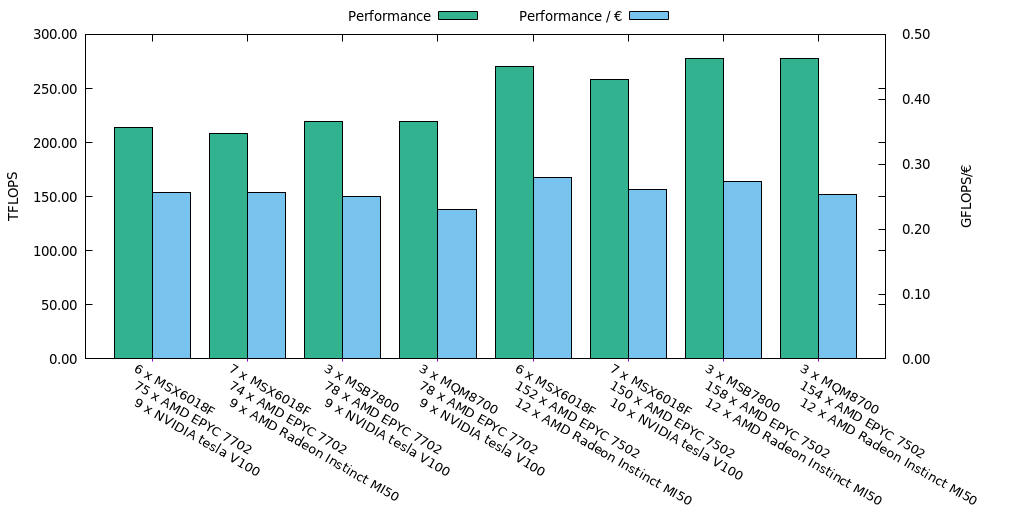
\includegraphics[width=\textwidth]{img/summary}
    \caption{Gràfica de les mètriques de rendiment de les combinacions de nodes valorades.}
    \label{fig:summary}
\end{figure}

En primer lloc, analitzem la taula \ref{tab:summary} en l'eix horitzontal. S'observa que els TFlops que ens garanteix utilitzar 3 commutadors de 36 ports i 3 de 40 són els mateixos. Això és degut a que amb els commutadors de 36 ports ja aconseguim connectar tots els nodes que ens caben en els racks, i per tant augmentar el nombre de ports disponibles no ens permet afegir més nodes; la limitació és el nombre de Us. La millora d'utilitzar els commutadors de 40 ports és que tenen una velocitat més bona, 200 Gbits en comptes de 100. El preu puja, però ens ho podem permetre.

Per altra banda, observem que amb 6 commutadors de 18 ports aconseguim una eficiència GFlops/Dòllar més bona, tot i que no arribem a tants TFlops com amb altres opcions.

Analitzant la taula \ref{tab:summary} en l'eix vertical, veiem que per qualsevol configuració la versió amb dual-socket ens dóna més TFlops amb una eficiència econòmica millor. Això pot ser degut en part a que els nodes amb gràfiques poden tenir-ne fins a vuit per node en comptes de quatre com en el cas del single-socket. Per tant, podem tenir més gràfiques utilitzant menys U, deixant-ne més disponibles per a nodes sense gràfiques (1 U).

